\subsection{Placa triangular horizontal}
El procedimiento para hallar el momento de inercia de una placa triangular
delgada (véase la \textbf{Figura \ref{figura11}}) con eje en el centro de masa y
perpendicular a sus medidas ($a$, $b$), es el siguiente:

\begin{figure}
\centering
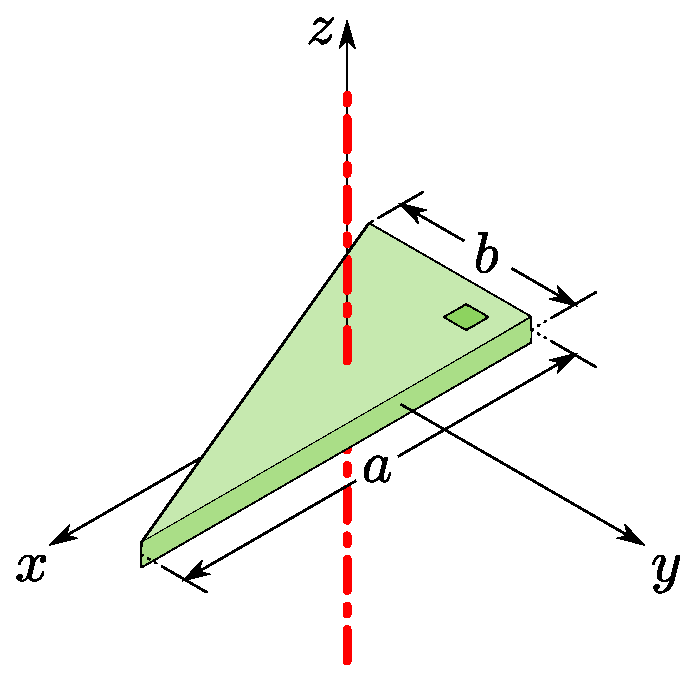
\includegraphics[scale=0.5]{resources/f11.eps}
\caption{Placa triangular horizontal.}
\label{figura11}
\end{figure}

Considerando la \textbf{Ecuación (\ref{solidorigido})}:

\begin{equation*}
    I = \int_{M} r^2\, dm
\tag{4}
\end{equation*}

Asumiendo la distribución homogénea y superficial de la masa:

\begin{equation*}
    \sigma = \frac{dm}{ds} = \frac{dm}{dx\, dy}
\end{equation*}

Por tanto:

\begin{equation}
    dm = \sigma\, dx\, dy
\label{dm7}
\end{equation}

Considerando la relación trigonométrica entre $r$, $x$, $y$:

\begin{equation}
    r^2 = x^2 + y^2
\label{r7}
\end{equation}

Calculando la ecuación de la recta que conforma la hipotenusa del triangulo a
partir de las coordenadas $P_1 = (\frac{2}{3} a, \frac{1}{3} b)$ y
$P_2 = (- \frac{1}{3} a, - \frac{2}{3} b)$:

\begin{equation*}
    \frac{y - y_1}{x - x_1} = \frac{y_2 - y_1}{x_2 - x_1}
\end{equation*}
\begin{equation*}
    \frac{y - \frac{1}{3} b}{x - \frac{2}{3} a} = \frac{- \frac{2}{3} b - \frac{1}{3} b}{- \frac{1}{3} a - \frac{2}{3} a}
\end{equation*}
\begin{equation*}
    \frac{3y - b}{3x - 2a} = \frac{b}{a}
\end{equation*}
\begin{equation*}
    3ya - ab = 3bx - 2ab
\end{equation*}
\begin{equation*}
    y = \frac{b}{a} x - \frac{1}{3} b
\end{equation*}

Reemplazando (\ref{r7}) y (\ref{dm7}) en (\ref{solidorigido}):

\begin{equation*}
    I = \int_{M} r^2\, dm = \int_{-\frac{1}{3} a}^{\frac{2}{3} a} \int_{\frac{b}{a} x - \frac{1}{3} b}^{b/3} (x^2 + y^2)\, \sigma\, dy\, dx = \sigma\, \int_{-\frac{1}{3} a}^{\frac{2}{3} a} \int_{\frac{b}{a} x - \frac{1}{3} b}^{b/3} (x^2 + y^2)\, dx \, dy
\end{equation*}
\begin{equation*}
    I = \sigma\, \int_{-\frac{1}{3} a}^{\frac{2}{3} a} \left( \int_{\frac{b}{a} x - \frac{1}{3} b}^{b/3} x^2 dx + \int_{\frac{b}{a} x - \frac{1}{3} b}^{b/3} y^2 dx \right) \, dy = \sigma\, \int_{-\frac{1}{3} a}^{\frac{2}{3} a} \left( \frac{x^3}{3} \Biggr|_{\frac{b}{a} x - \frac{1}{3} b}^{b/3} + y^2 x \Biggr|_{\frac{b}{a} x - \frac{1}{3} b}^{b/3} \right) \, dy
\end{equation*}
\begin{equation*}
    I = \sigma\,
\end{equation*}

\subsection{Placa triangular vertical}
El procedimiento para hallar el momento de inercia de una placa rectangular
delgada (véase la \textbf{Figura \ref{figura12}}) con eje en el centro de masa,
paralelo a su medida ($b$) y perpendicular a su media ($a$), es el siguiente:

\begin{figure}
\centering
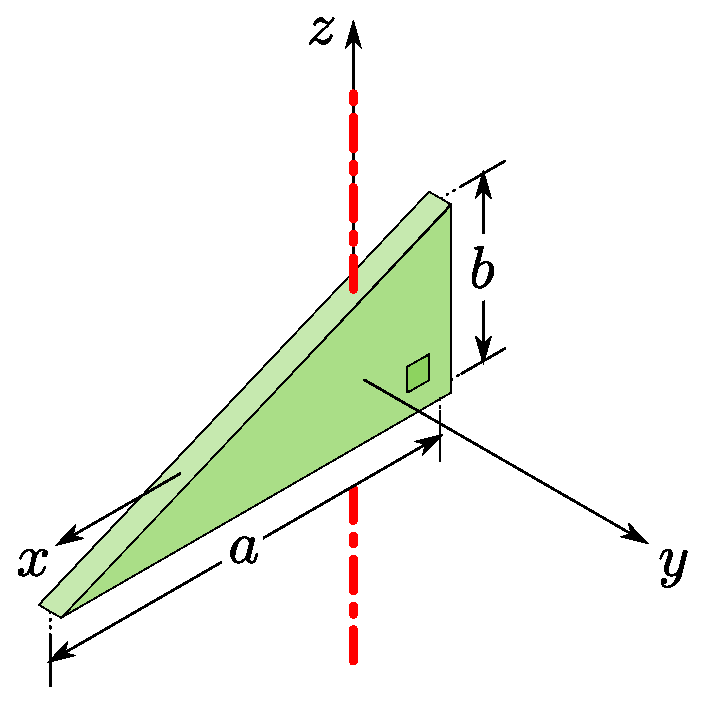
\includegraphics[scale=0.5]{resources/f12.eps}
\caption{Placa rectangular vertical.}
\label{figura12}
\end{figure}

\subsection{Cono horizontal}
El procedimiento para hallar el momento de inercia de un cono solido
(véase la \textbf{Figura \ref{figura19}}) con eje en el centro de masa,
perpendicular a su radio ($R$) y paralelo a su altura ($h$), es el siguiente:
 
\begin{figure}
\centering
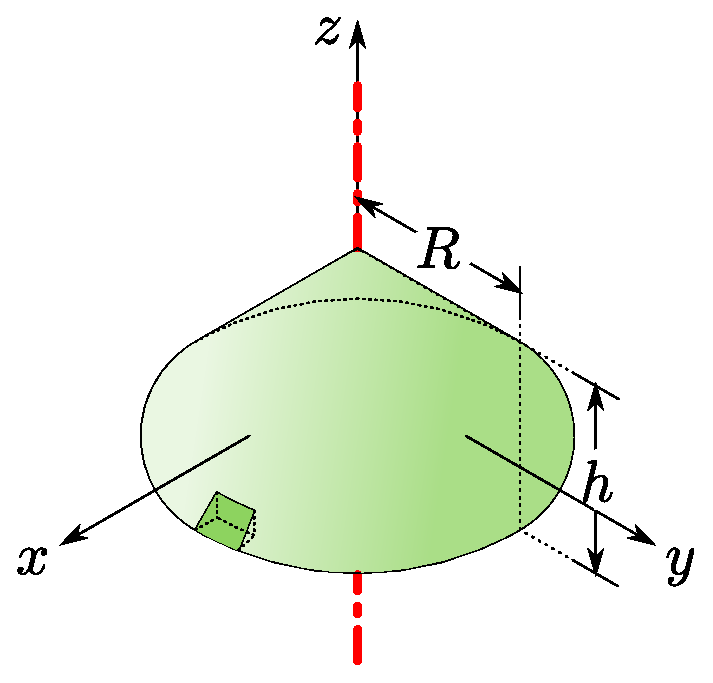
\includegraphics[scale=0.5]{resources/f19.eps}
\caption{Cono horizontal.}
\label{figura19}
\end{figure}

\subsection{Cono vertical}
El procedimiento para hallar el momento de inercia de un cono solido
(véase la \textbf{Figura \ref{figura20}}) con eje en el centro de masa,
paralelo a su radio ($R$) y perpendicular a su altura ($h$), es el siguiente:

\begin{figure}
\centering
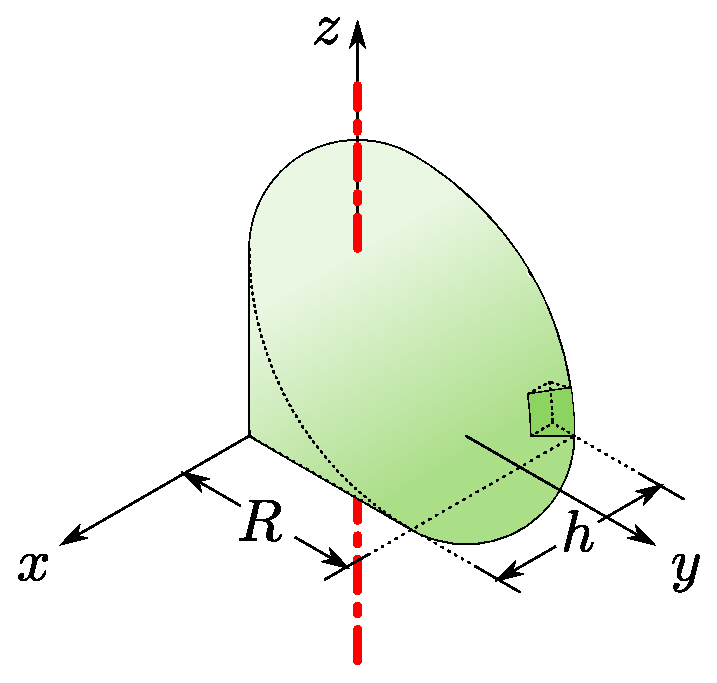
\includegraphics[scale=0.5]{resources/f20.eps}
\caption{Cono vertical.}
\label{figura20}
\end{figure}

